% FermiSets architecture figure — FermiNet-style redraw (data = vertical vector
% blocks, operations = labeled arrows between them), matching plots/thesis/IMG_2964.JPG.
%
% Notation, reconciled against three sources simultaneously:
%   - Fu 2025 (arXiv:2510.11431): symmetric feature xi(R), signature encoder eta(R),
%     lifted function Psi odd in eta (their Eqs. 2, 4-6) -- the Psi_0 / antisymmetrize
%     steps below, matching src/ansatz.py's eval_psi0()/log_psi0_plus/minus naming.
%   - Zaheer et al. 2018 (Deep Sets, arXiv:1703.06114), already cited in the thesis --
%     phi = per-element network, rho = post-pool network, xi(R) = rho(sum_i phi(x_i))
%     is literally their defining equation; no other gloss is used for phi/rho.
%   - src/ansatz.py FermiSets: phi_dense1/2, rho_dense1, eta_antisymmetric, Psi_dense1/2.
%
% Vectors are drawn either as a 2-cell stack (a genuinely low-dim quantity: a
% coordinate, eta, or a complex log-amplitude) or as a tall solid bar labeled
% with its real dimension (64, 66 at the canonical benchmark,
% configs/experiment/qho_fermisets_2d_3N_bench.yaml). The fanned/offset copies
% at the input and after phi mark "one such vector per particle, shared
% weights", collapsing to a single vector only after the Sigma pool -- the
% same repeated-stream convention the FermiNet paper's own figure uses.
%
% Deliberately NOT shown: the internal safe-complex-logsumexp reductions
% (inside Psi_0's readout, and in how the antisymmetrizing combine is actually
% computed) -- numerically-stable ways to *compute* the formula below, not
% part of the architecture; and any trap-specific envelope -- this figure
% characterises the ansatz itself (Fu's construction + Deep Sets), which is
% potential-independent, not the QHO-specific implementation.
%
% Compiles standalone:  pdflatex fermisets_architecture.tex
% Thesis use: \input the tikzpicture body into a figure environment (inherits
% your document's font), or \includegraphics the resulting .pdf directly.
\documentclass[tikz,border=4pt]{standalone}
\usepackage{amsmath}
\usepackage{amssymb}
\usetikzlibrary{positioning, arrows.meta, matrix, backgrounds, calc}

% Okabe-Ito colorblind-safe palette: blue for the xi (symmetric) branch, orange
% for the eta (antisymmetric) branch. Everything else stays black/grey.
\definecolor{symblue}{RGB}{0,114,178}
\definecolor{antiorange}{RGB}{230,159,0}
\definecolor{inkgrey}{RGB}{60,60,60}

% fan-of-copies decoration behind an already-placed node NODE, tinted COLOR,
% indicating "one such vector per particle" (or, with a single light copy,
% "evaluated twice"). Draw AFTER the node exists; renders behind it regardless.
\newcommand{\fan}[2]{
  \begin{scope}[on background layer]
    \draw[thick, draw=#2!70, fill=#2!6]  ($(#1.south west)+(2.0mm,2.0mm)$) rectangle ($(#1.north east)+(2.0mm,2.0mm)$);
    \draw[thick, draw=#2!70, fill=#2!10] ($(#1.south west)+(1.0mm,1.0mm)$) rectangle ($(#1.north east)+(1.0mm,1.0mm)$);
  \end{scope}
}
\newcommand{\fantwo}[2]{
  \begin{scope}[on background layer]
    \draw[thick, draw=#2!70, fill=#2!10] ($(#1.south west)+(1.2mm,1.2mm)$) rectangle ($(#1.north east)+(1.2mm,1.2mm)$);
  \end{scope}
}

\begin{document}
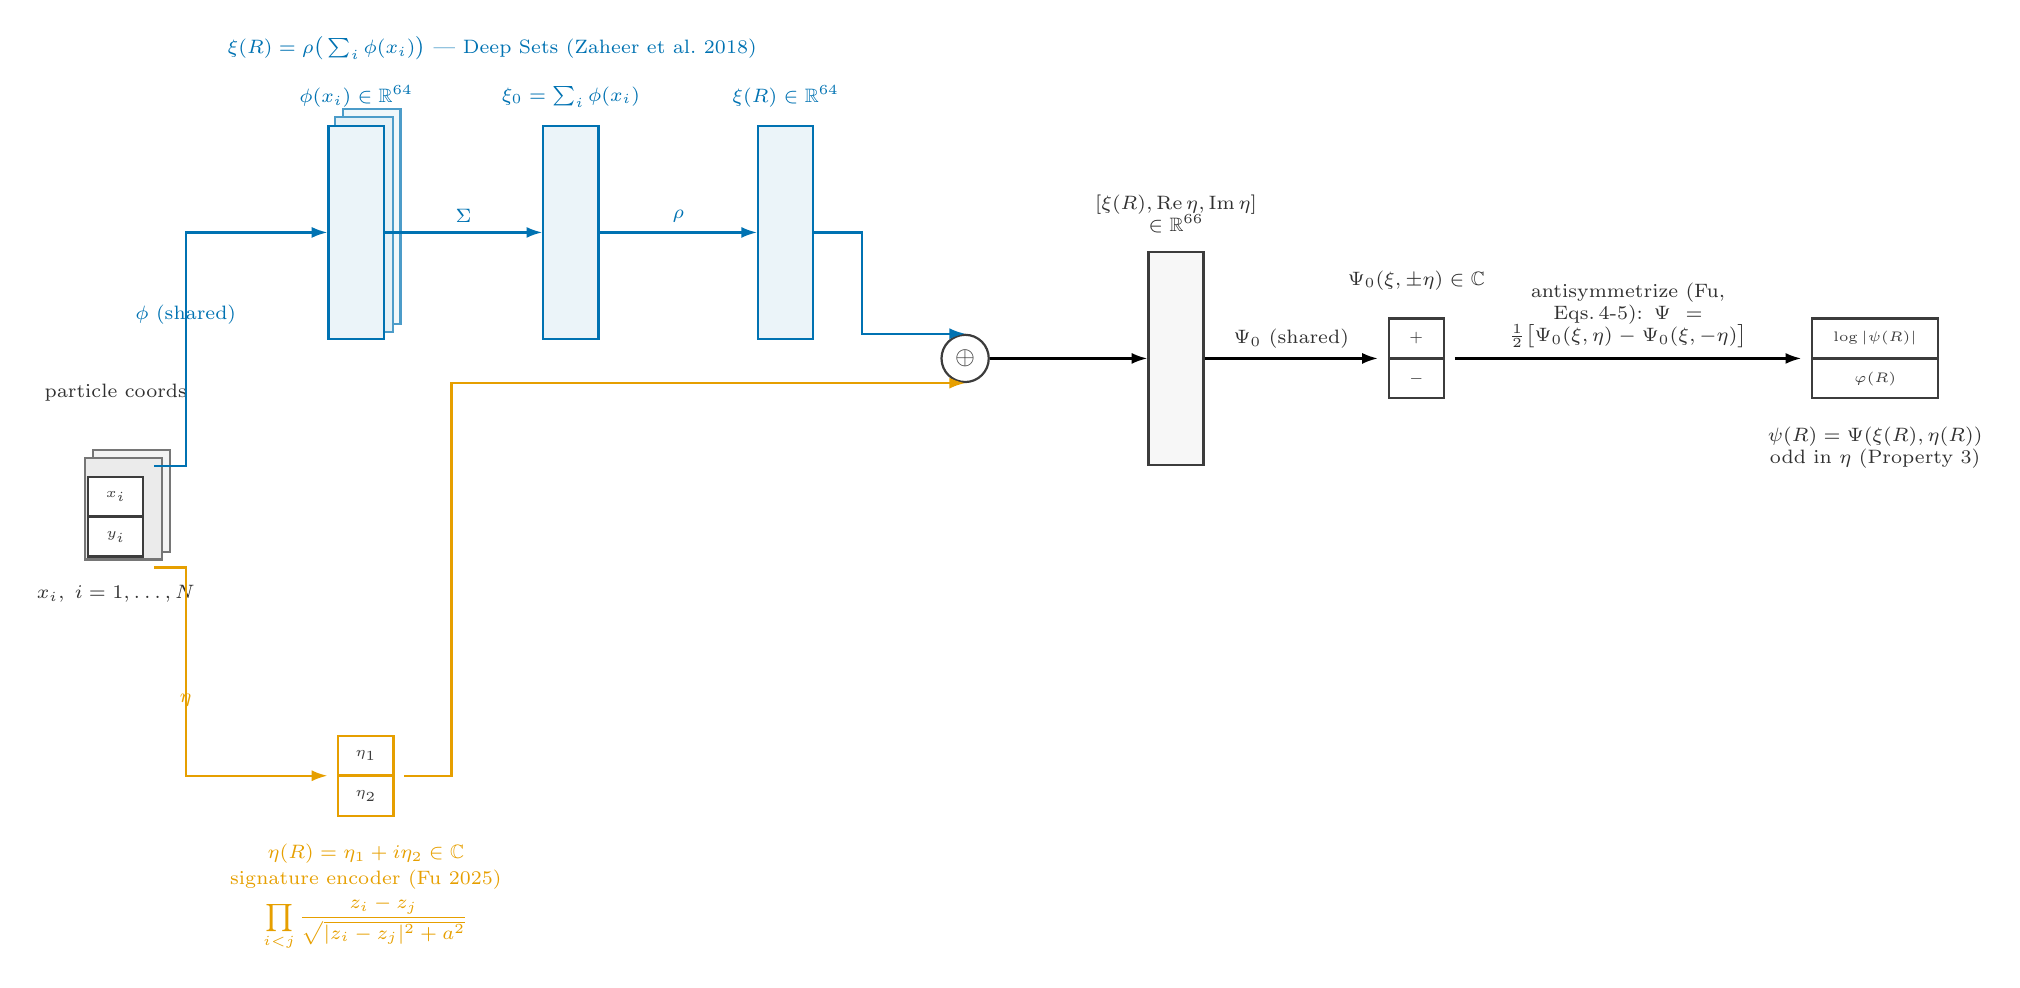
\begin{tikzpicture}[
    font=\small,
    >={Latex[length=2mm,width=1.4mm]},
    every node/.style={text=inkgrey},
    cell/.style={draw=inkgrey, thick, minimum width=7mm, minimum height=5mm, inner sep=0pt, fill=white, font=\tiny},
    symcell/.style={cell, draw=symblue},
    anticell/.style={cell, draw=antiorange},
    vec2/.style={matrix of nodes, nodes={cell}, row sep=-\pgflinewidth, ampersand replacement=\&},
    vec2sym/.style={matrix of nodes, nodes={symcell}, row sep=-\pgflinewidth, ampersand replacement=\&},
    vec2anti/.style={matrix of nodes, nodes={anticell}, row sep=-\pgflinewidth, ampersand replacement=\&},
    bar/.style={draw=inkgrey, thick, minimum width=7mm, minimum height=27mm, inner sep=0pt, fill=inkgrey!4},
    symbar/.style={bar, draw=symblue, fill=symblue!8},
    lbl/.style={font=\scriptsize, text=inkgrey!80!black},
    symlbl/.style={lbl, text=symblue},
    antilbl/.style={lbl, text=antiorange},
    arrow/.style={-{Latex[length=2mm,width=1.4mm]}, thick},
    symarrow/.style={arrow, symblue},
    antiarrow/.style={arrow, antiorange},
]

% ---------------------------------------------------------------- input ---
\matrix[vec2] (xin) {$x_i$ \\ $y_i$ \\};
\fan{xin}{inkgrey}
\node[lbl, above=7mm of xin] {particle coords};
\node[lbl, below=1mm of xin] {$x_i,\;i=1,\dots,N$};

% ------------------------------------------------------- xi branch (top) ---
\node[symbar, above right=16mm and 22mm of xin] (phi) {};
\fan{phi}{symblue}
\node[symlbl, above=1mm of phi] {$\phi(x_i)\in\mathbb{R}^{64}$};
\draw[symarrow] (xin.north east) -- ++(4mm,0) |- node[pos=0.28, above, symlbl] {$\phi$ (shared)} (phi.west);

\node[symbar, right=20mm of phi] (xi0) {};
\node[symlbl, above=1mm of xi0] {$\xi_0=\sum_i\phi(x_i)$};
\draw[symarrow] (phi) -- node[above, symlbl] {$\Sigma$} (xi0);

\node[symbar, right=20mm of xi0] (xi) {};
\node[symlbl, above=1mm of xi] {$\xi(R)\in\mathbb{R}^{64}$};
\draw[symarrow] (xi0) -- node[above, symlbl] {$\rho$} (xi);

\node[symlbl, above=7mm of xi0, xshift=-10mm, font=\scriptsize]
  {$\xi(R)=\rho\big(\textstyle\sum_i\phi(x_i)\big)$ — Deep Sets (Zaheer et al.\ 2018)};

% --------------------------------------------------- eta branch (bottom) ---
\matrix[vec2anti, below right=20mm and 22mm of xin] (eta) {$\eta_1$ \\ $\eta_2$ \\};
\draw[antiarrow] (xin.south east) -- ++(4mm,0) |- node[pos=0.28, below, antilbl] {$\eta$} (eta.west);
\node[antilbl, below=1mm of eta, align=center]
  {$\eta(R)=\eta_1+i\eta_2\in\mathbb{C}$\\[0.5mm]signature encoder (Fu 2025)\\[0.5mm]
   \scriptsize$\displaystyle\prod_{i<j}\frac{z_i-z_j}{\sqrt{|z_i-z_j|^2+a^2}}$};

% ---------------------------------------------------------- concatenate ---
\node[draw=inkgrey, thick, circle, minimum size=6mm, right=16mm of xi, yshift=-16mm, inner sep=0pt] (concat) {$\oplus$};
\draw[symarrow] (xi.east) -- ++(6mm,0) |- (concat.north);
\draw[antiarrow] (eta.east) -- ++(6mm,0) |- (concat.south);

\node[bar, right=20mm of concat] (cat) {};
\node[lbl, above=1mm of cat, align=center] {$[\xi(R),\mathrm{Re}\,\eta,\mathrm{Im}\,\eta]$\\$\in\mathbb{R}^{66}$};
\draw[arrow] (concat) -- (cat);

% --------------------------------------------------- Psi_0, shared, +-eta ---
\matrix[vec2, right=22mm of cat] (psi0) {$+$ \\ $-$ \\};
\node[lbl, above=1mm of psi0, align=center] {$\Psi_0(\xi,\pm\eta)\in\mathbb{C}$};
\draw[arrow] (cat) -- node[above, lbl, align=center, pos=0.5] {$\Psi_0$ (shared)} (psi0);

% ------------------------------------------------------- antisymmetrize ---
\matrix[vec2, right=44mm of psi0, nodes={cell, text width=16mm, align=center}] (psi) {$\log|\psi(R)|$ \\ $\varphi(R)$ \\};
\draw[arrow] (psi0) -- node[above, lbl, align=center, text width=34mm, pos=0.5]
  {antisymmetrize (Fu, Eqs.\,4-5): $\Psi=\tfrac12\big[\Psi_0(\xi,\eta)-\Psi_0(\xi,-\eta)\big]$} (psi);
\node[lbl, below=1mm of psi, align=center] {$\psi(R)=\Psi(\xi(R),\eta(R))$\\odd in $\eta$ (Property 3)};

\end{tikzpicture}
\end{document}
